\chapter{Materials and methodologies}\label{cap: Material_method}
In this section there's going to be an explanation of the dataset as well as instruments and methodologies used to analyze it's properties, as such the first step is going to be an in depth discussion of the data available and a general overview of the final use. The following step is going to be a description of the preliminary work done to the data itself and to the results of this preliminary analysis in order to select the important features. The final step of this chapter is going to be an explanation of the methods used to derive the final results and to evaluate them.


\section{Data and objective}
\label{chap:freefree}
The objective of this thesis will be to compare how different methods perform in predicting clinical outcomes in covid patients, while also determining if different kind of input data imply different performances of the same methods.
%The main focus is going to be on clinical images, i.e. lung CTs, used in conjunction with clinical and laboratory labels which are obtainable as soon as the patient is admitted in the hospital facilities. All clinical images are going to be analysed through the lens of radiomics while all clinical labels are provided as is by clinical professionals.
All images are non segmented, as such all of them have been semi-automatically segmented via a new software being tested in the medical physics department called \textit{Sophia Radiomics}  which seems to be built around region growth algorithm mixed with thresholding. 

Statistical analysis are going to be performed mainly in python using libraries such as scikit-learn, pandas, numpy, scipy while the graphical part of the analysis is done with either seaborn or matplotlib.

The starting dataset was a list of all the patients that, from 02/2020 to 05/2021, were hospitalized as COVID-19 positive inside the facilities of \textit{Azienda ospedaliero-universitaria di Bologna - Policlinico Sant'Orsola-Malpighi}. 

As far as exclusion criteria go the main deciding factors, except unavailability of the feature related to the patient, were visibly damaged and lower quality images, for example images with cropped lungs. The first set of selection criteria were:

\begin{itemize}
\item All patients that had undergone a CT exam which was retrievable via the PACS (Picture Archiving and Communication System) of \textit{Azienda ospedaliero-universitaria di Bologna - Policlinico Sant'Orsola-Malpighi}
\item All patients that had a all of the clinical and laboratory features, listed in fig:\ref{fig:ClinicalFeatures}, suggested by medical professionals.
\item Since all patient had at least 2 CT exams only the closest date to the hospital admission date was taken. When more exams were performed on the same date all of them were initially taken. At first only chest or abdomen CTs were taken regardless of the acquisition protocol used.
\end{itemize}

\begin{figure}[H]
  		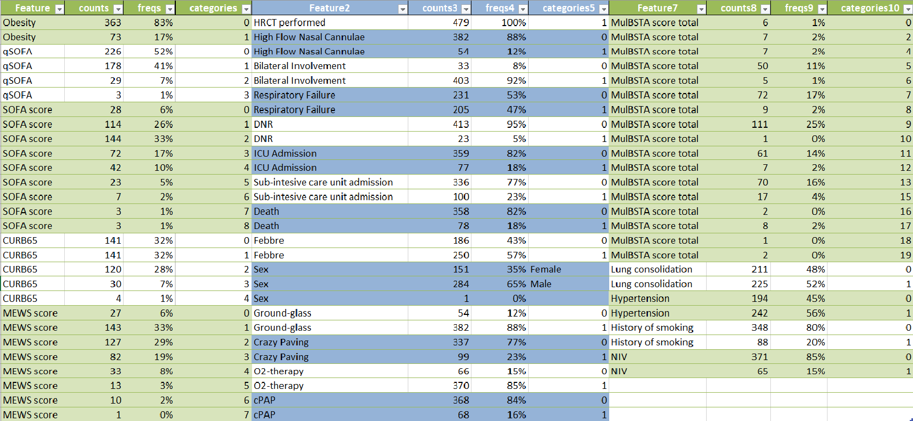
\includegraphics[width=1\textwidth]{Clinical_Feature_Description.png}
        \caption{Description of clinical label dataset, in sets of four columns there's the clinical feature, the total count of occurences, the percentage over the final dataset and the possible values the feature could take \todo[inline]{usare excel come immagine non è il massimo}\label{fig:ClinicalFeatures}}
\end{figure}

%Most clinical features are pretty self-explanatory, for those that were obscure to me as an outsider and not otherwise explained in \ref{Clinical_Covid_Manifestations}, I'm going to provide a very simple explanation:
Most clinical features are pretty self-explanatory, a brief explanation will be provided for those that could appear obscure to an outsider, and that were not explained in \ref{Clinical_Covid_Manifestations}.

\begin{enumerate}\label{clinical_features}
\item DNR : Acronym for "Do Not Resuscitate", used to indicate the wish of the patient or their relatives that cardiac massage not be performed in case of cardiac arrest.
\item NIV: Acronym for "Non Invasive Ventilation", it's a form of respiratory aid provided to patients.
\item cPAP: Acronym for  "continuous Positive Airway Pressure", another form of respiratory aid.
\item ICU: Acronym for "Intensive Care Unit". When patients are in really severe conditions they are treated in these facilities.
\item Clinical Scores: When available values from laboratory analyses and/or patient conditions are summarised in scores that represent the gravity of the state of the patient, as such these can be somewhat correlated and could be treated as comprehensive values to substitute an otherwise large set of obscure clinical features. At admission, or closely thereafter, a set of clinical questions regarding the patient receives a yes or no answer, each answer has an additive contribution towards the final value of the score.

These scores differ in how much they add for each condition and the set of symptoms the check for.
	\begin{enumerate}
		\item MulBSTA: This score acconts for \textbf{Mul}tilobe lung involvement, absolute \textbf{L}ymphocyte count, \textbf{B}acterial coinfection, history of \textbf{S}moking, history of hyper\textbf{T}ension and \textbf{A}ge over 60 yrs. \cite{MulBSTA}
		\item MEWS: Modified Early Warning Score for clinical deterioration. Computed considering systolic blood pressure, heart rate, respiratory rate, temperature and AVPU(Alert Voice Pain Unresponsive) score. \cite{MEWS}
		\item CURB65: \textbf{C}onfusion, blood \textbf{U}rea Nitrogen or Urea level, \textbf{R}espiratory Rate, \textbf{B}lood pressure, age over \textbf{65} years. This score is specific for pneumonia severity \cite{CURB65}
		\item SOFA:  \textbf{S}equential  \textbf{O}rgan  \textbf{F}ailure  \textbf{A}ssessment score. Considers various quantities from all systems to assess the overall state of the patient, PaO$_2$/FiO$_2$\footnote{Very unrefined yet widely used indicator for lung disfunction} for respiratory system, Glasgow Coma scale\footnote{GCS for short, proposed in 1974 by Graham Teasdale and Bryan Jennet. Evaluates what kind of stymulus is necessary to obtain motor and verbal reactions in the patient as well as what's necessary for the patient to open their eyes} for nervous, mean pressure for cardiovascular, Bilirubin levels for liver, platelets for coagulation and creatine for kidneys \cite{SOFA}
		\item qSOFA:  \textbf{q}uick SOFA. Only considers pressure, high respiratory rate and the low values in the Glasgow scale.
	\end{enumerate}
\end{enumerate}

\begin{figure}
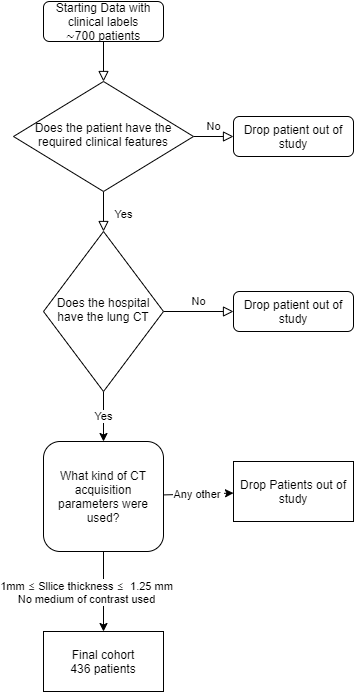
\includegraphics[width=\textwidth]{Data_flowchart.png}
\caption{Flowchart of the patient selection procedure \label{fig:dataSelFlowchart}}
\end{figure}

This procedure produced a starting cohort of $\sim$700 patients which, having all various images available, created a huge set of $\sim$2200 CT scans. Since this analysis is focused on radiomics there is an evident need for as much consistency as possible in the images analysed. For this reason all CTs taken with medium of contrast were excluded, since they would have brightnesses not indicative of the disease, and for every patient only images with thin slice reconstruction were considered. 

More specifically only images with slice thickness of 1 o 1.25 mm
\footnote{This meant that only exams called 'Parenchima' or  'HRCT' were included. Throughout the internship 'parenchima' has always appeared in contrast with 'mediastino'. These two keywords are used in the phase of reconstruction of the raw data to identify reconstructions with specific properties. Parenchima is used for finer reconstruction of lung specifically, the requiring professional uses these images to look for small nodules with very high contrast and, to do so, the reconstruction allows some noise to achieve the best resolution possible. Mediastino is used in the lung, as well as other regions, to look for bigger lesions but with low contrast. As such the 'mediastino' reconstruction compromises a worse spatial resolution for a better display of contrast, visually speaking the first images are more coarse and noisy while the second are smoother. It should be noted that even with the same identifier, be it HRCT parenchima or others, the machines on which the exams were made were different and had different proprietary convolutional kernels used for reconstruction.} 
along the z-axis were taken into consideration, which meant excluding all the 1.5,2,2.5 and 5 mm slice thicknesses.

All images were segmented using a tool provided by \orsola.
\todo[inline]{Per dott.ssa Strigari: Metto il nome del programma? Va citato in qualche modo particolare?}

Overall this left the final study cohort to be composed of 434 patients, all descriptions and analyses are related to this cohort.

The same software used for segmentation allowed the extraction of the radiomic features form the segmented volumes, even if it did not allow the extraction of the segmentation masks nor any changes in the segmentation parameters. For this reason all the image analysis in this thesis is reliant on said software which has been treated as a black-box.

So, having segmented all the images and extracted all the features supported in the software, the next step is the definition of the actual analysis pipeline. The whole dataset was comprised of $\sim$200 features, which were divided in three subgroups as follows:

\begin{enumerate}
\item Clinical: All these features are derived from the admission procedure in the hospital.
	\begin{itemize}
        \item The continuous are {\scshape age taken at the date of the CT exam} and {\scshape respiratory Rate} defined as number of breaths in a minute.
		\item The discrete one were the aforementioned scores and the boolean ones were {\scshape sex of the patient, obesity status, if the patient had a fever}\footnote{Defined as body temperature$>$38°} as of hospital admission and whether or not the patient suffered of {\scshape Hypertension}
		\item The remaining features, namely those in \ref{clinical_features} as well as the \death status of the patient, were either used as labels or not used at all because they refer to treatments used and not characteristics of the patient. As such these features, while plausibly correlated to the clinical outcome, are not really descriptive of the patient as of admission and are not information that can be used to aid professionals at admission to assess the situation
	\end{itemize}
\item Radiomic: These features were all the ones supported by the segmentation software and are pretty much most of those described in \cite{IBSI} with the addition of fat and muscle surface, computed as cm$^2$ by counting pixel identified via threshold as fat or muscle tissue in thoracic slices taken at height of vertebra T-12
\item Radiological: These features are those that can be derived from CT exams by humans. Namely acquisition parameters, such as {\scshape KVP} and {\scshape Current}, were used to search for eventual correlations between image quality and predictive power of the feature derived from the image while boolean features, such as {\scshape Bilaterality} of lung damage, presence of {\scshape Ground Glass Opacities (GGO)}, {\scshape lung consolidations} as well as {\scshape crazy paving} were used to see if they were sufficient in determining outcome.
\end{enumerate}

\section{Preprocessing and data analysis}
\begin{figure}
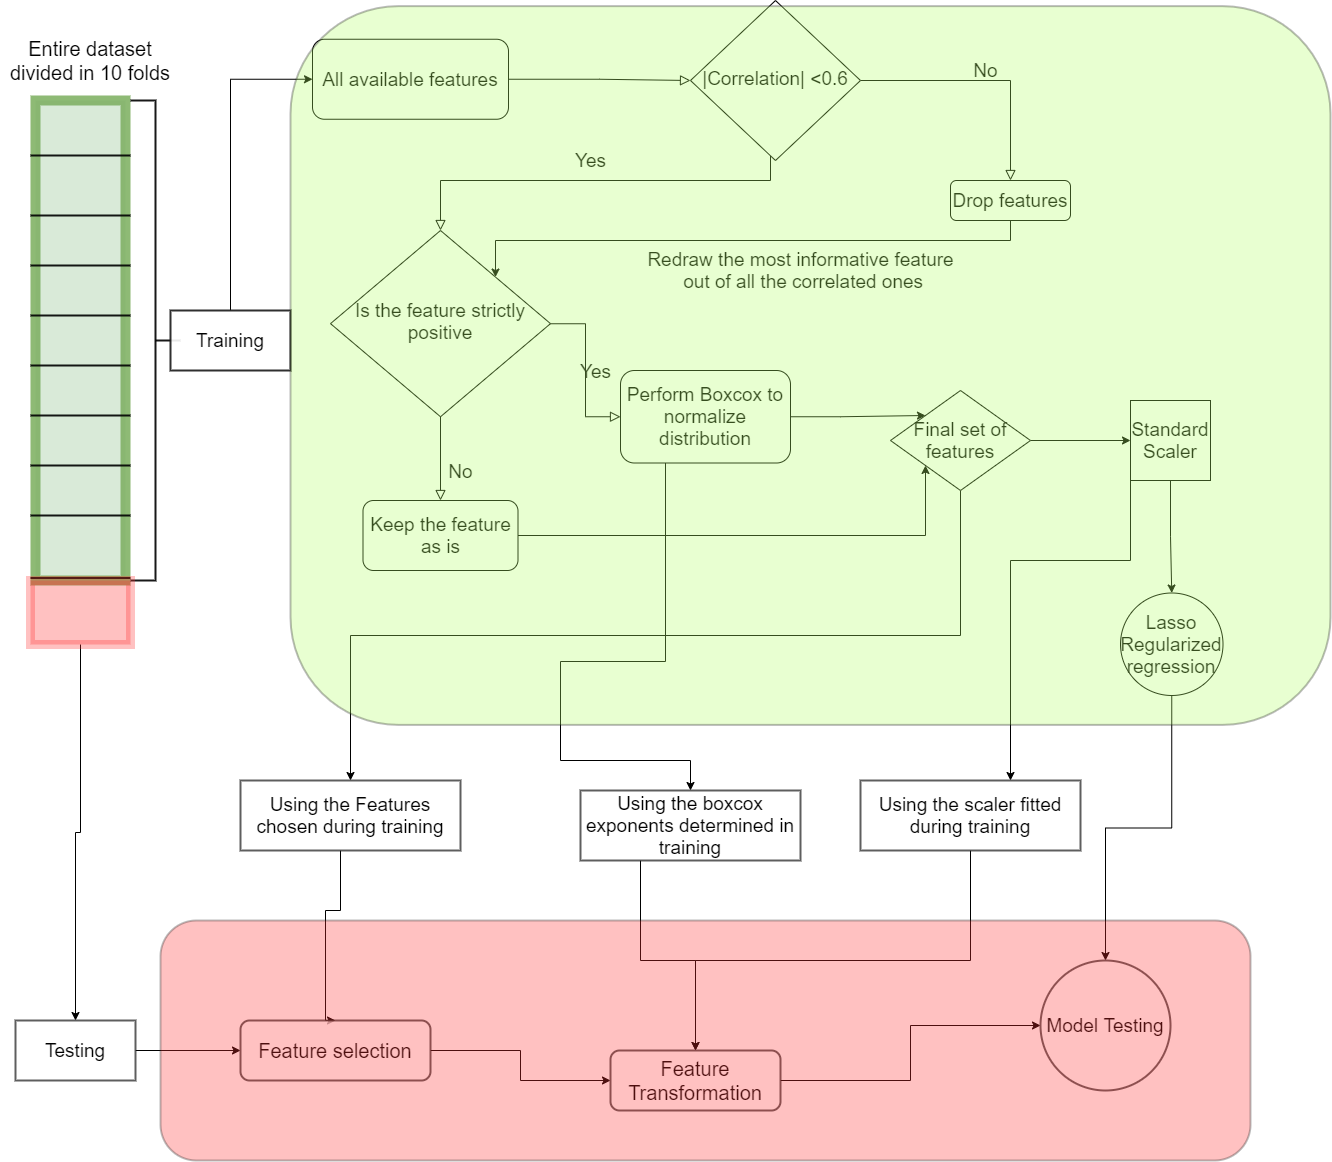
\includegraphics[width=\textwidth]{Preprocessing_flowchart.png}
\caption{Flowchart for the preprocessing steps before preceeding a Lasso regularized regression. \label{fig:preprocFlowchart}}
\end{figure}

Before any preprocessing a choice was made to exclude all of the clinical scores, this was done to avoid having them mask other, more straightforward variables.

The first step in the analysis of this data is going to be a lasso regularized regression using either \death or \icu as target. As mentioned before when operationg with regressions it's a necessity that the residuals be normally distributed, a common way to get as close as possible to this hypothesis is to boxcox transform the data. Apart from the data which contained negative values, which cannot be fed into the boxcox transform, all variables have been transformed using this method.

\begin{figure}[htbp]
  		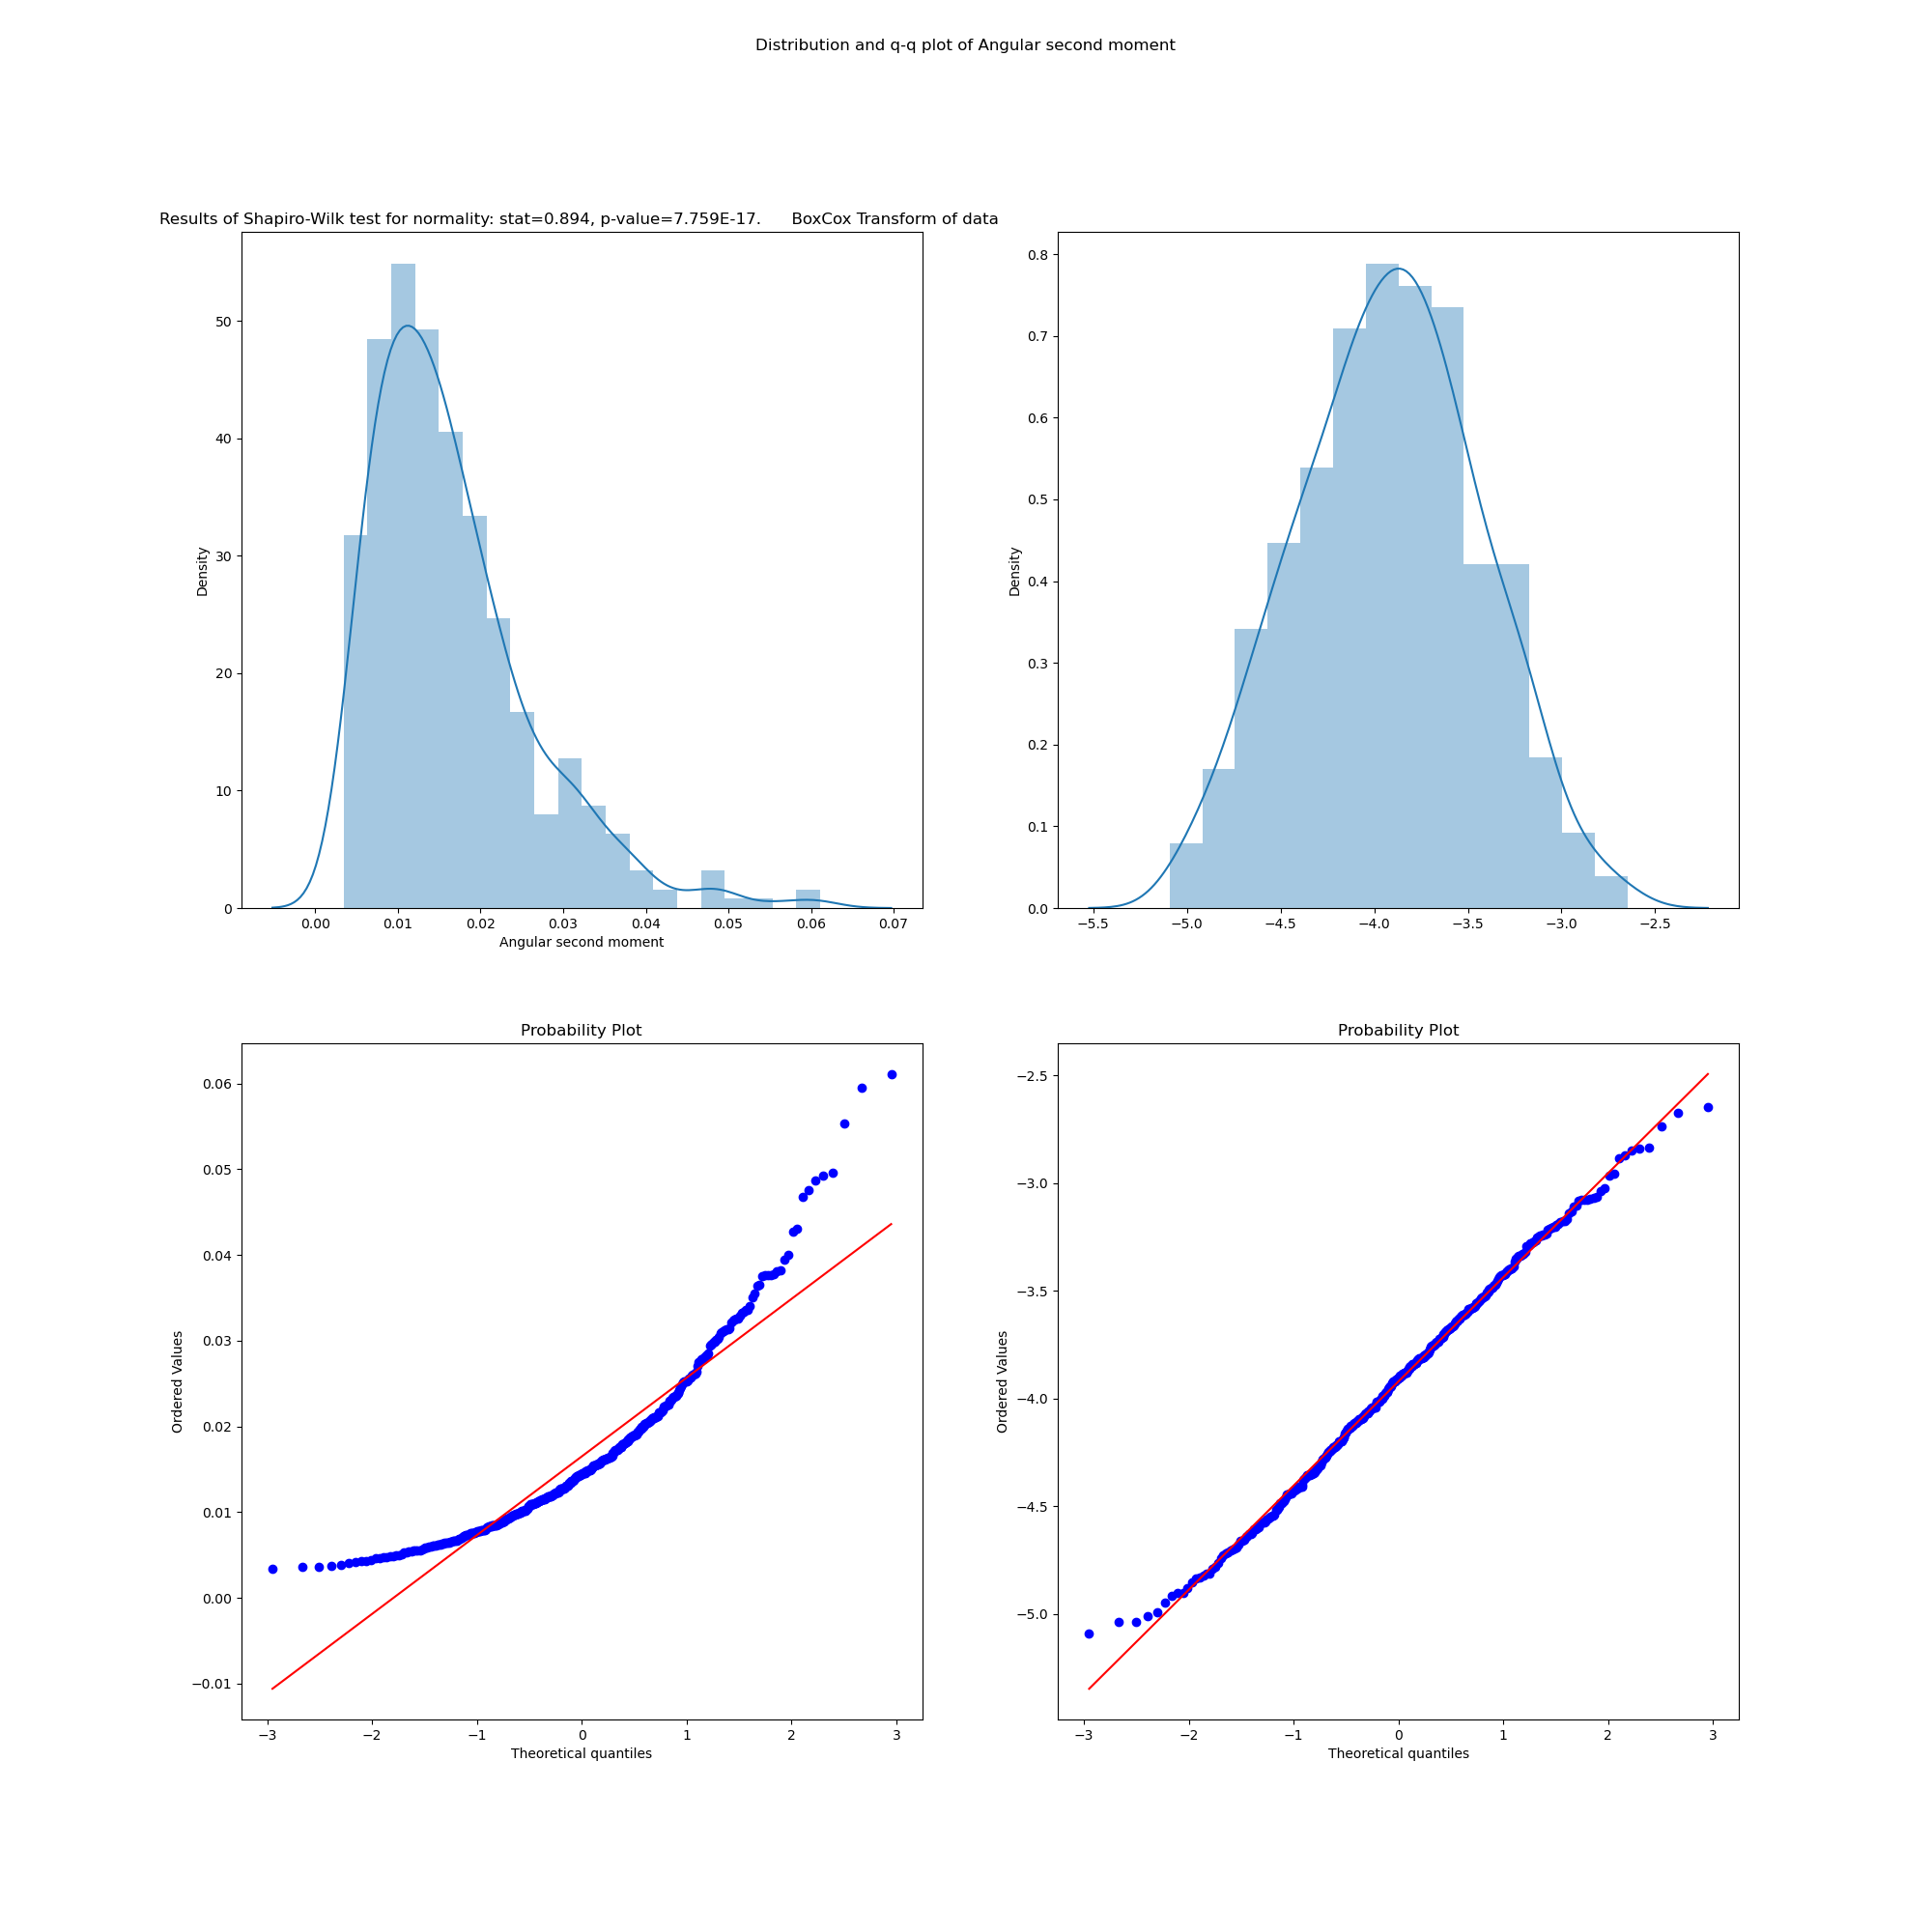
\includegraphics[width=1\textwidth]{distribution_Angular_second_moment.png}
        \caption{Example of boxcox applied to the radiomic feature \textit{Angular second moment} which has a heavy tailed distribution. The graphs contain the original distribution (top-left) the transformed distribution (top-right) and the two respective quantile-quantile plots(bottom) \label{fig:boxcox_example}}
\end{figure}

\begin{figure}[htbp]
  		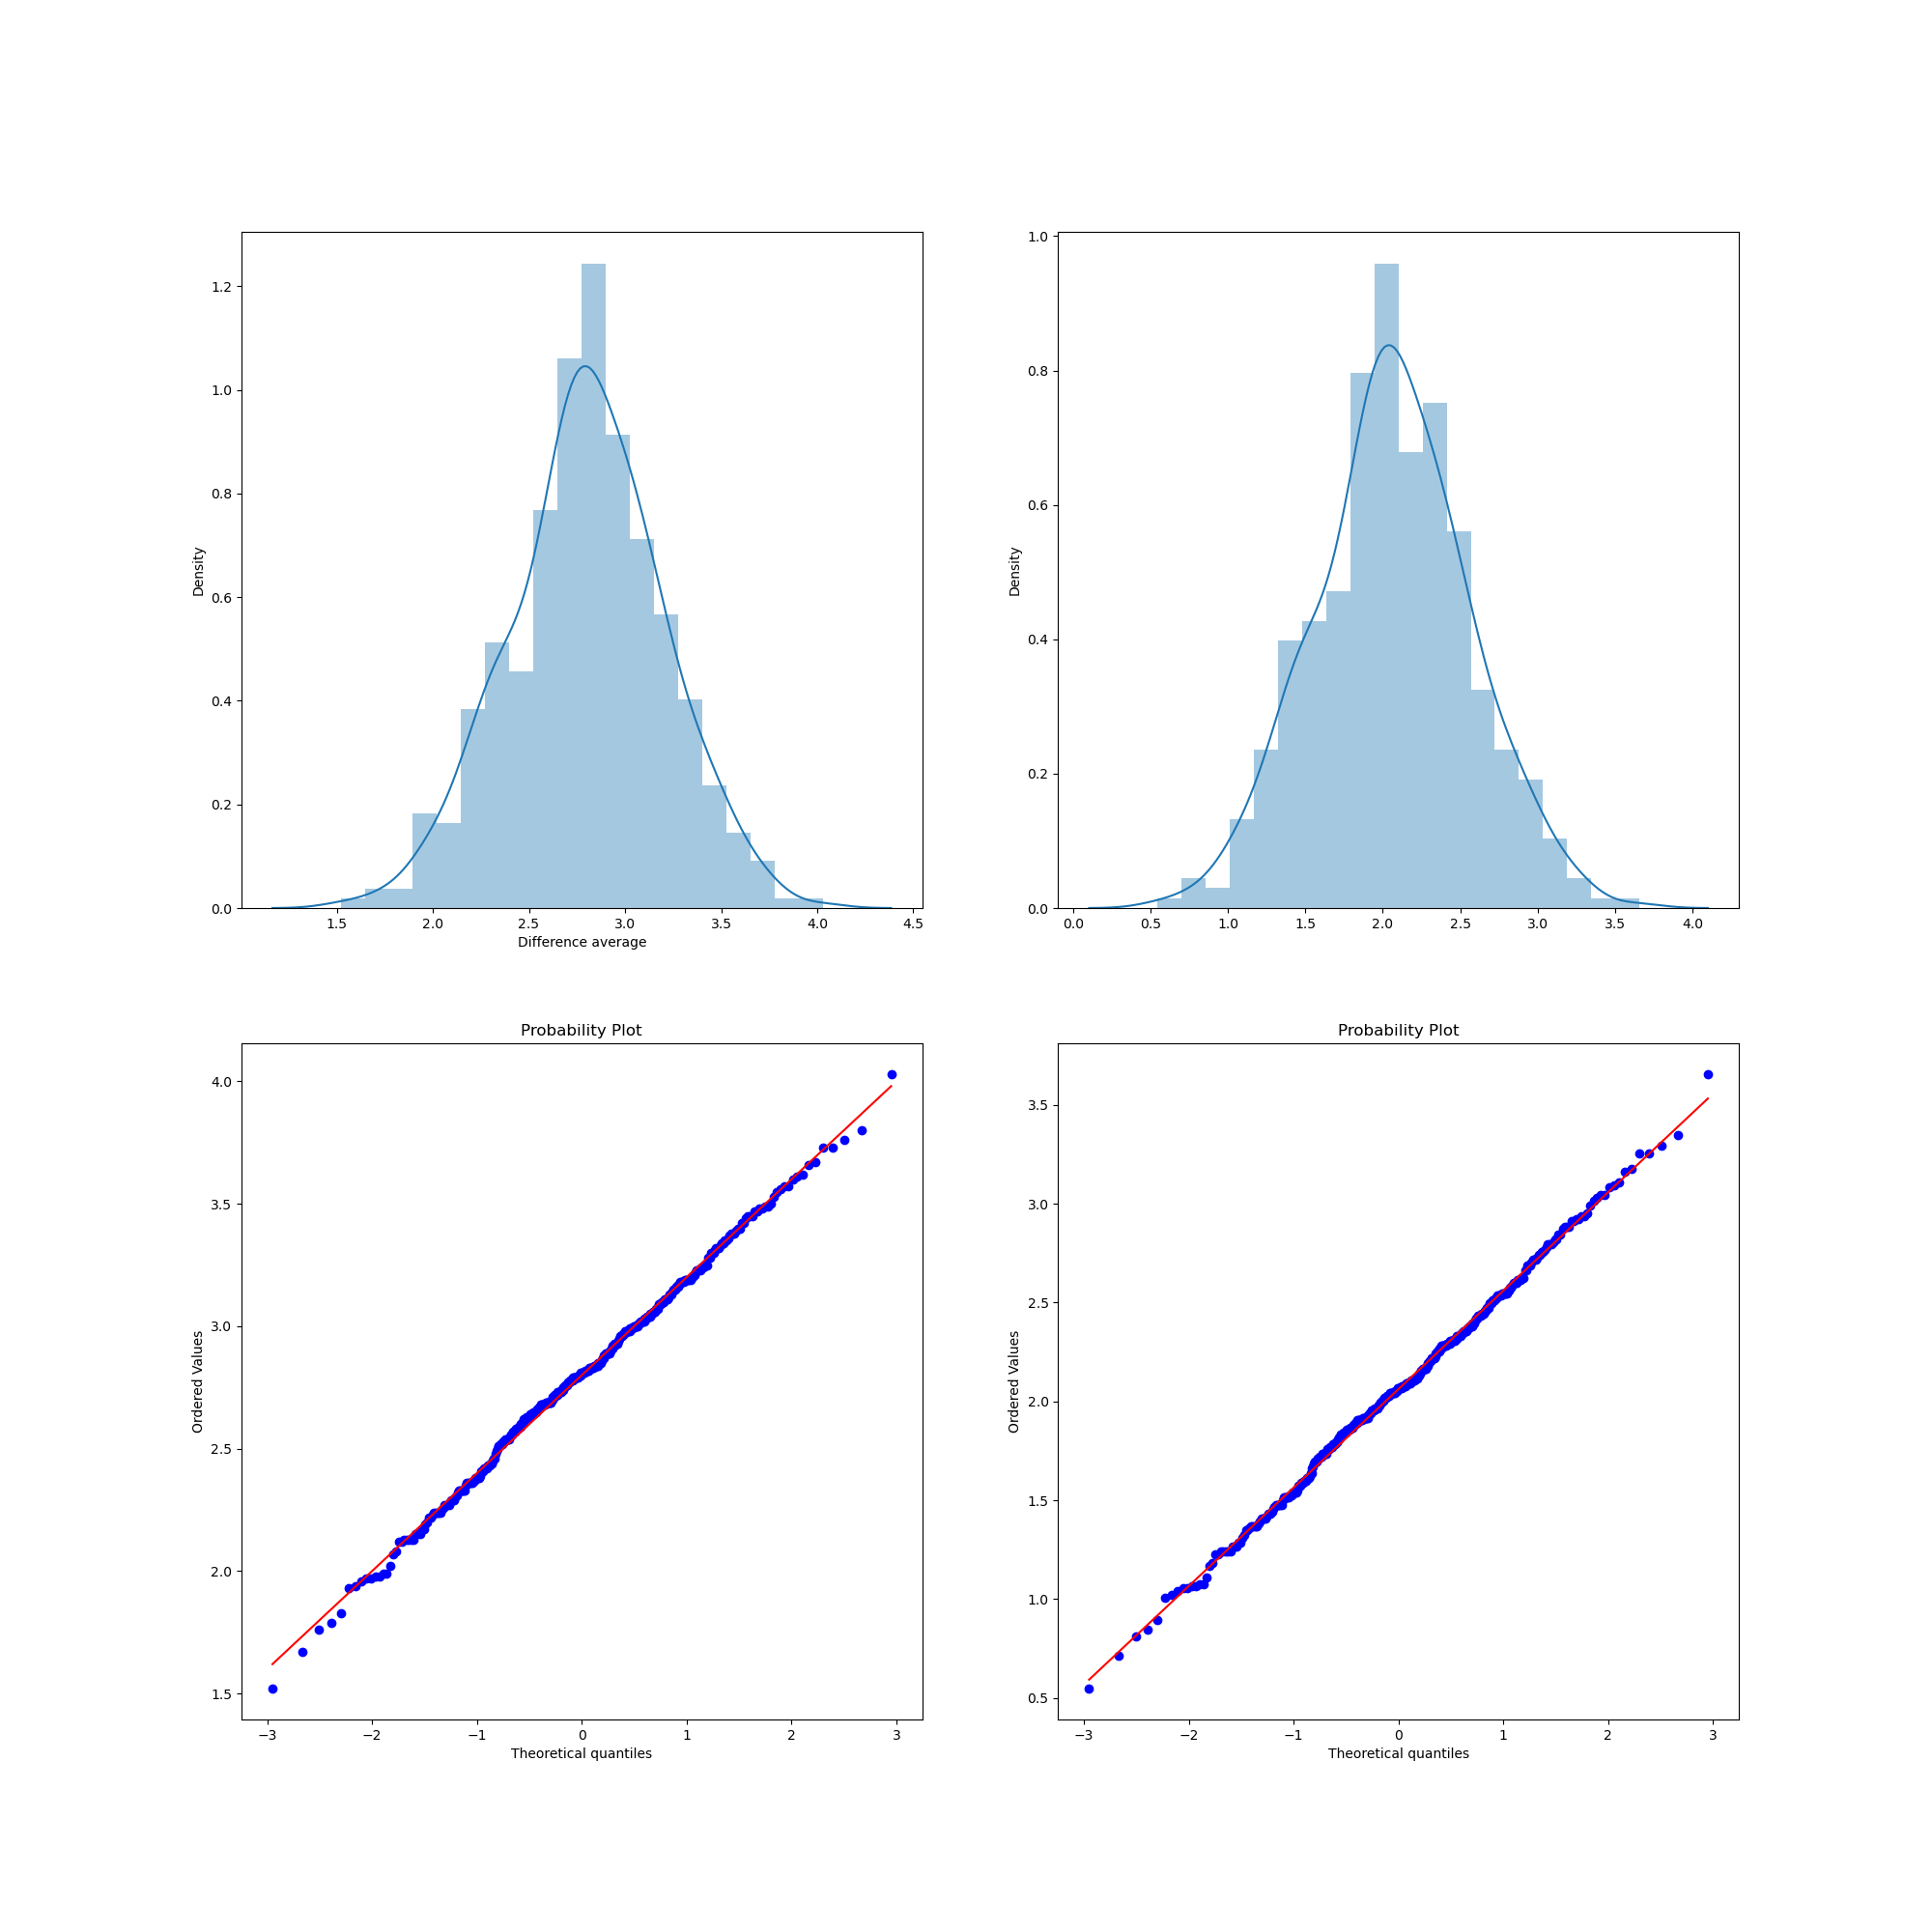
\includegraphics[width=1\textwidth]{distribution_Difference_average.png}
        \caption{Example of boxcox applied to the radiomic feature \textit{Difference Average} which has a close to normal distribution. The graphs contain the original distribution (top-left) the transformed distribution (top-right) and the two respective quantile-quantile plots(bottom) \label{fig:boxcox_example_normal}}
\end{figure}

The quatile-quantile plots have been used for a visual check of normality, normally distributed data will populate the bisector of the graph while deviations are symptoms of non-normality. Heavy and light tails are visible as deviations respectively above and belox the bisector.

 It should be noted that when the data is normally distributed then the transform doesn't change much the distribution while, in cases with more heavy tailed distributions, the improvement is clear to see as it can be seen in Figures \ref{fig:boxcox_example} and \ref{fig:boxcox_example_normal}.

The next preprocessing step has been to apply a \textit{StandardScaler} to all of the features, which corresponds to subtracting the mean and dividing by the standard deviation, in order to center all the features around zero. 

The final step in preprocessing has been to reduce the features by using a correlation threshold which means that all variables that correlate with another more, in absolute value, than a certain threshold, which has been set to 0.6 in this work, are dropped a priori. A rather important thing to notice is that correlation has been computed using Spearman correlation and not Pearson since the first is invariant under monotone transformations, such as boxcox, and the second is not.

Given the large number of features it's very plausible that at least one of the eliminated features is correlated with all other dropped features but with none of the remaining ones, since a Lasso regularization will be used introducing a few redundant features is not too damaging and the possible benefits outweight the risks. For this reason a redrawing method has been implemented to add one of the dropped features, this has been done by choosing the one that most correlates with the label being used.

A pivotal point in all of this analysis is that, to obtain reasonable values in the cross-validation procedures and to avoid leakage\footnote{This term is used in the field of Machine Learning. It refers to models being created on information that comes from outside the training data.} problems, all of the preprocessing steps have been done after train-test splitting the data on the train set and then applied as defined during training on the test dataset.

When it comes to cross-validation procedure the choice was made to use a stratified k-fold approach with k=10. The data is split in 10 parts with the same percentages of labels\footnote{The stratified in the name refers to this property. This method is useful when dealing with unbalanced datasets, such the one under analysis, in which the label has an uneven 15-85$\%$ frequency of occurences of the two labels} then a model is built by training on 9 of the folds and it's performance is then tested on the remaining fold. To use the whole dataset for testing a prediction of it has been built by combinimg the predictions on the 10$^{th}"$ fold for ten different models trained on the respective 9 remaining folds.

The lasso model from training on the 9 folds is actually chosen as the model with the hyperparameters that give the best performance with another 10-fold crossvalidation. This has been obtained by using \textit{cross$\_$val$\_$predict} on a model obtained by including a \textit{LassoCV} step inside a \textit{pipeline} from scikit-learn library in python. 

The performance of the cross-validated predictions that, when built this way, is much more representative of the real-world performance of the model, has been evaluated using ROC curves and AUC.
Different models have been compared with a Delong test\cite{Delong} for the significance of difference in the ROC curves.

The second analysis method used was RandomForest. As said before in this case no preprocessing was needed nor has been done, however particular care was taken in handling the imbalances in the dataset by using SMOTE \cite{SMOTE} once again being careful to avoid leakage. 

The performance of this model was evaluated using confusion matrices which, at a glance, provide very much information on the situation of the data.
To facilitate the comparison of the results of the Random Forests with those obtained using Lasso regularized regression ROC curves were also made.

As a standalone method a Cox Proportional-Hazard model was used on the standard scaled variables remaining after the feature reduction performed through correlation thresholding. 
The score obtained with this procedure was then divided using different percentiles and tested using the log-rank test on Kaplan-Meier curves relative to the groups built.
In the case of this thesis the time variable was represented by the days of hospitalization computed using the dates of admission and discharge from the hospital provided by the hospital itself.
The idea of resorting to Kaplan-Meier curves was also used with other single variables to see if they had any effect. 

Finally a few dimensionality reduction techniques, namely the unsupervised PCA\cite{PCA} and Umap \cite{UMAP} and the supervised PLS-DA\cite{PLSDA}, have been used to understand better the state of the data and further explain some of the obtained results.
These peculiar analyses will be reported in the Appendix \todo[inline]{A seconda di come viene decisa la struttura finale questa frase va cambiata e aggiunta la reference al punto preciso}

This concludes the discussion on the methodologies used and leads perfectly in the discussion of the results.









